\chapter{Dokumentation des Projekverlaufs}
\section{Allgemeine Beschreibungen}
In unserer Diplomarbeit ist die Dokumentation der Arbeit wichtig und notwendig. Deswegen legen wir
besonders viel Wert auf die Dokumentation. Wir wollen n\"amlich, dass das, was wir machen, auch f\"ur andere erkl\"art und gut dokumentiert wird.


Die Webseite:
Damit die Leute in den ganzen Nord des Albaniens die Firma Kostandin Group Shkoder kennen, haben wir eine Webseite erstellt. Ihre Hauptfunktion ist Information \"uber die Firma zu geben. Man kann auch durch die Webseite die Adresse der Firma finden und hat auch einen SOS Funktion, um die Leute Hilfe von der Firma zu bekommen, wenn sie einen Problem mit ihrem Auto haben. In der Webseite kann man  auch \"uber die neue Angebote und andere Services sich informieren. \\

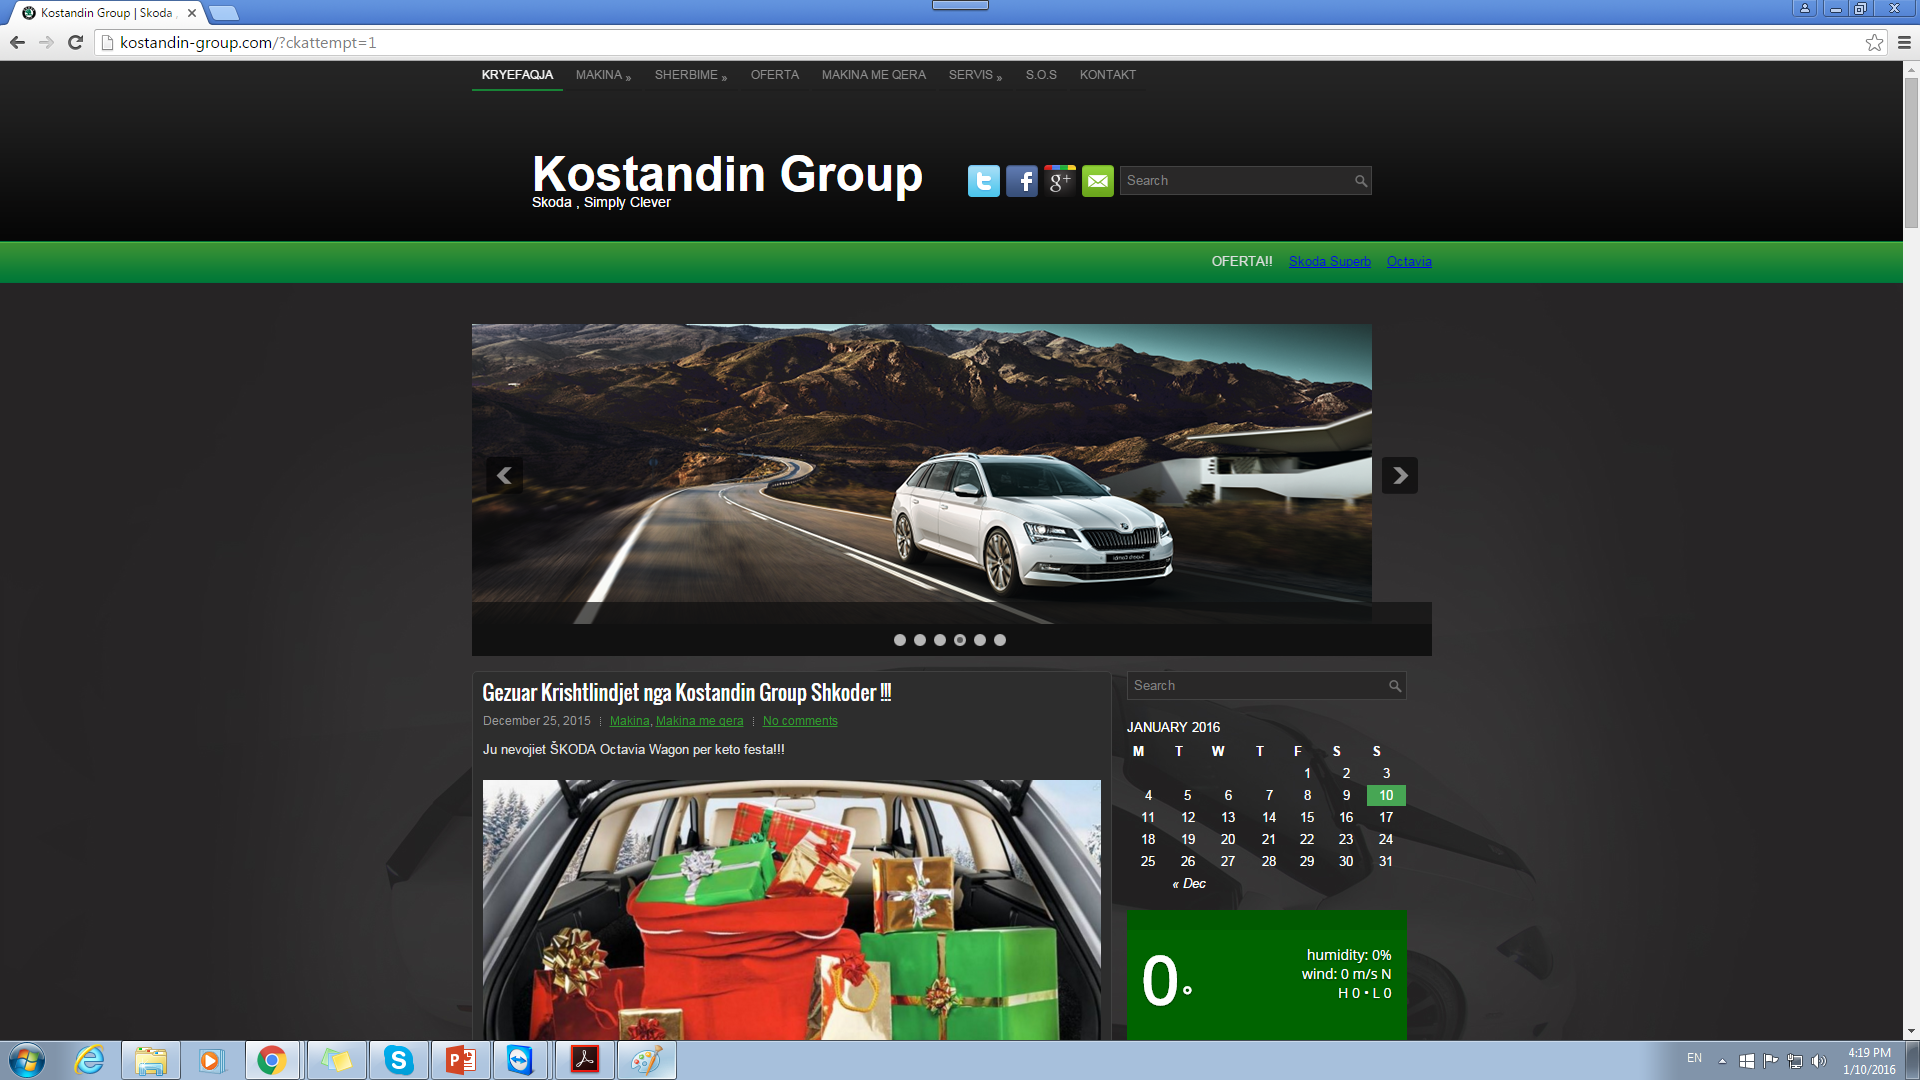
\includegraphics[scale=0.3]{Kryefaqja.png} \\
\\
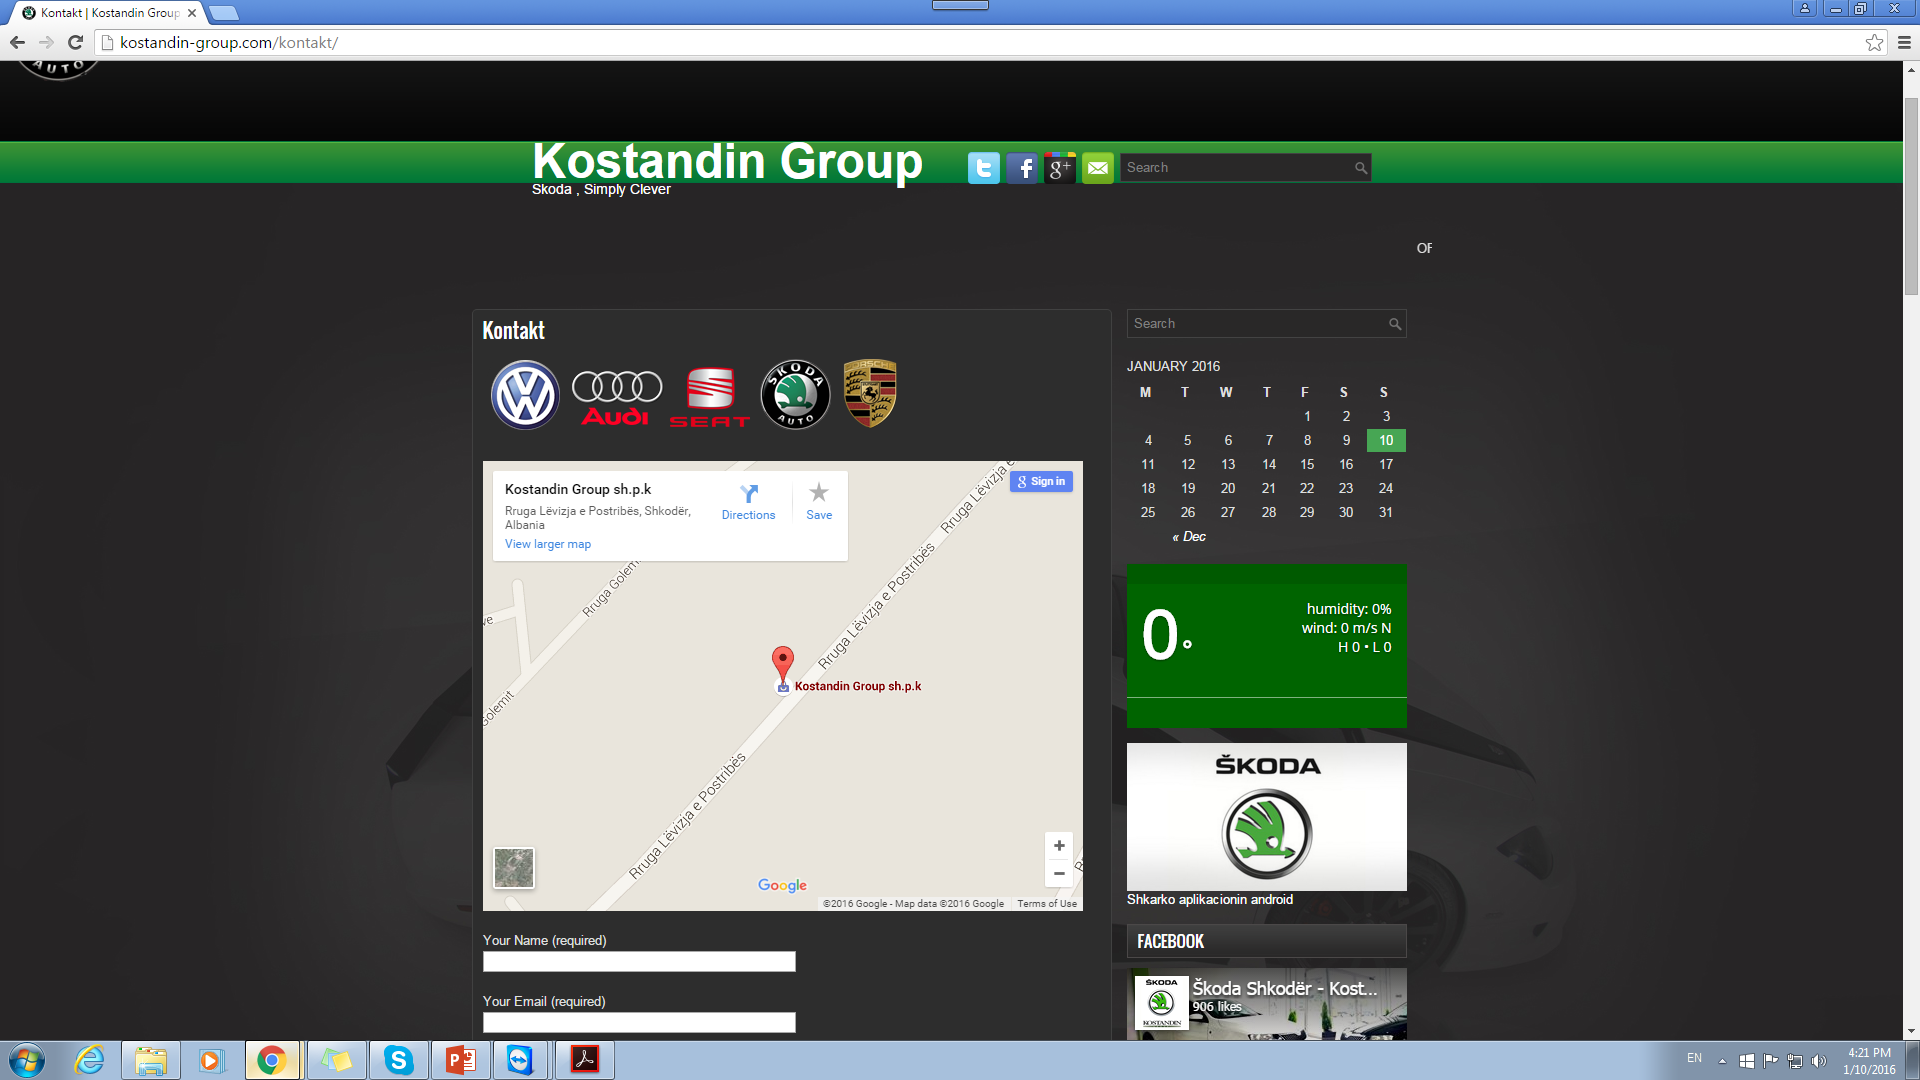
\includegraphics[scale=0.3]{Kontakt.png} \\
\\
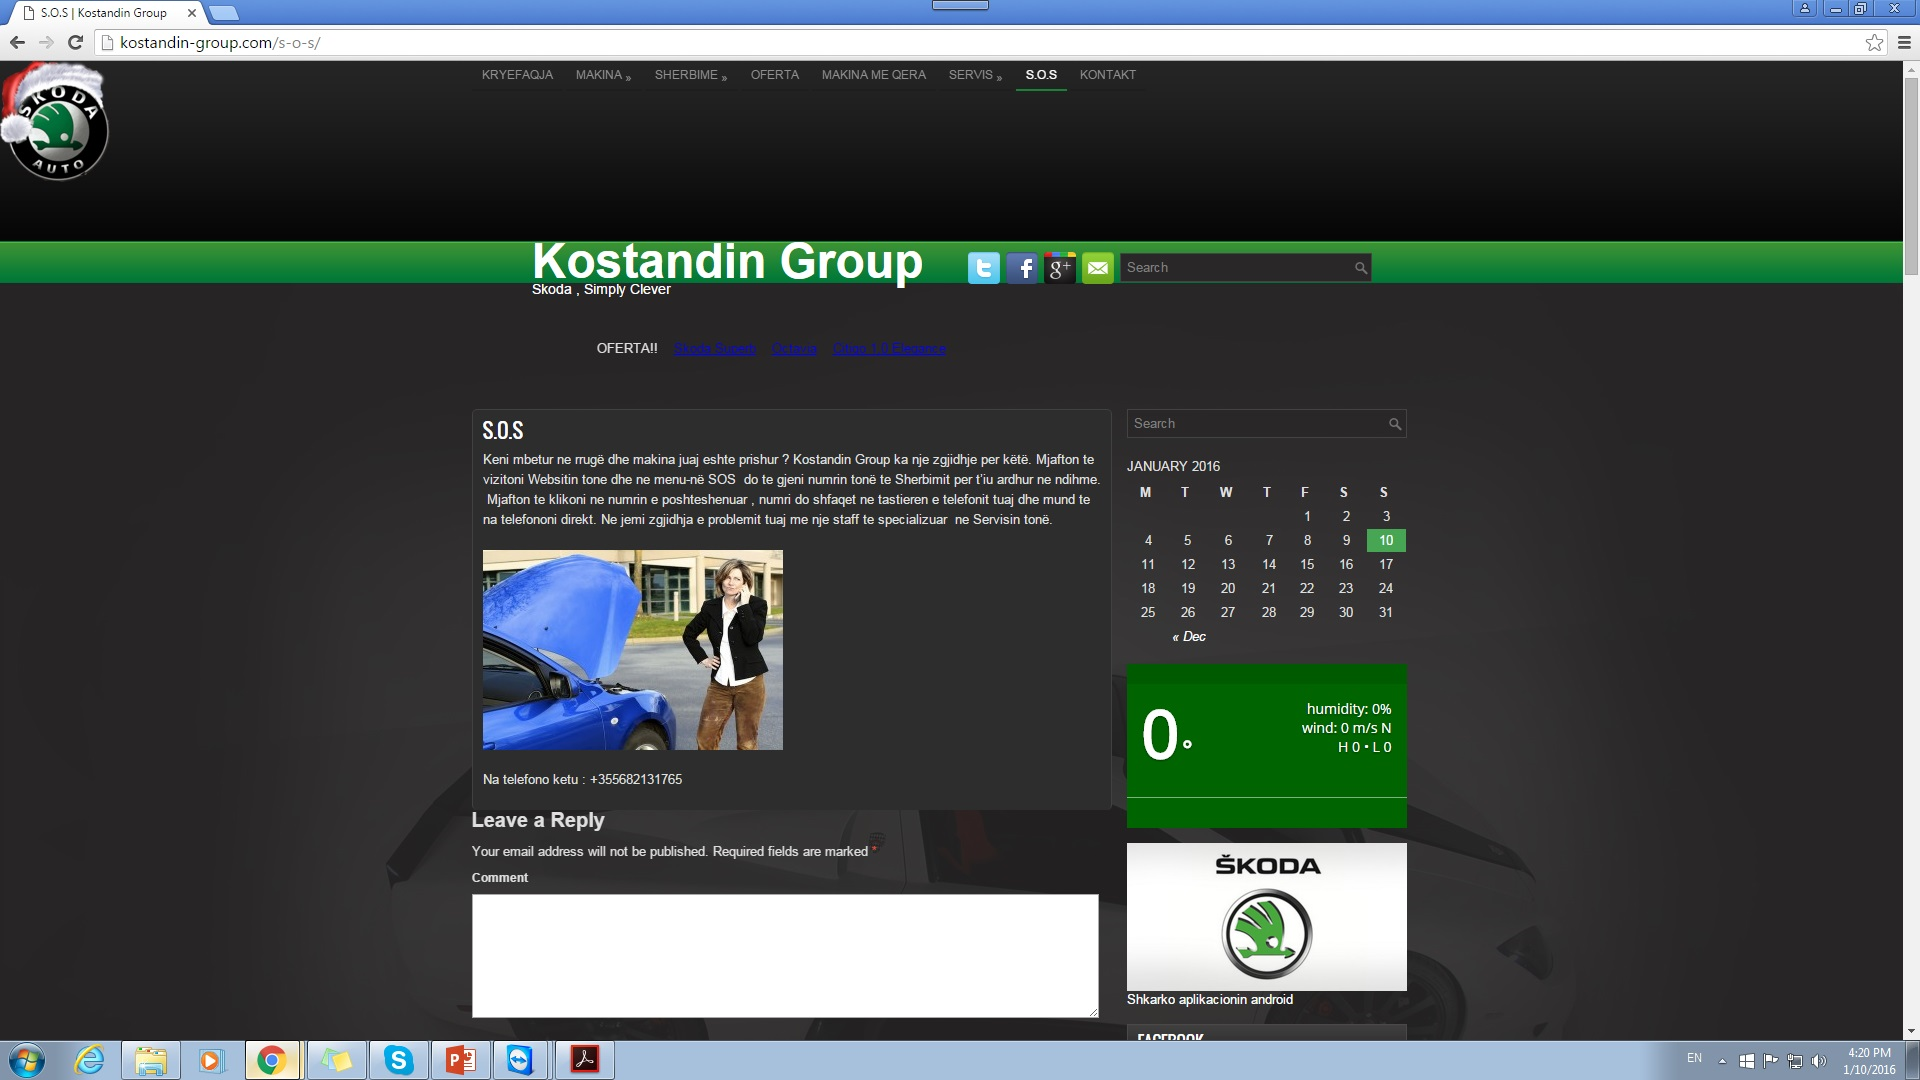
\includegraphics[scale=0.3]{SOS.png}



Die Hotspot-Zone:
Alle in Shkodra sollen wissen, wer 'Kostandin Group Skoda Shkoder' ist und was sie machen. Zu Werbezwecken wird f\"ur die Firma ein gratis Hotspot eingerichtet. Beim Verbinden mit dem Hotspot \"offnet sich als Startseite die aktuelle Firmenseite. Die Zone wo wir den Router eingesetzt haben ist in der Fussgangzone, eine Zone, die von viele Menschen jeden Tag frequentiert ist.

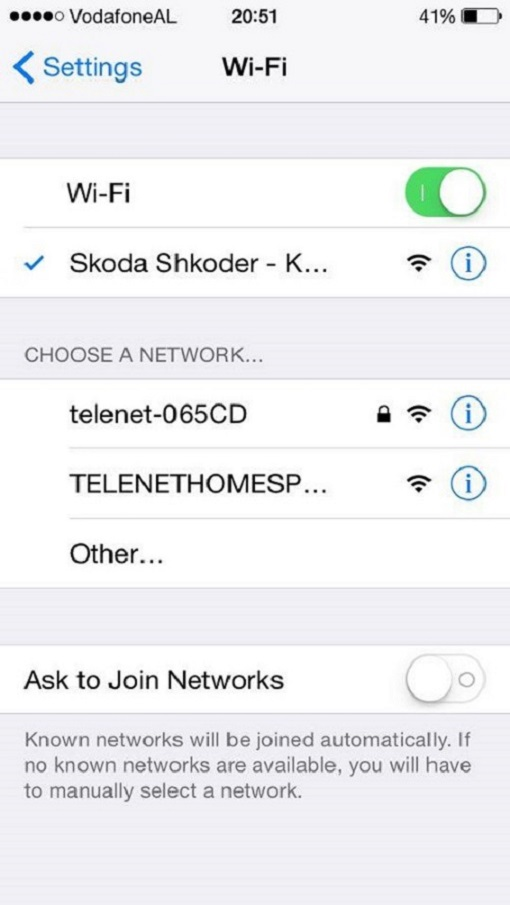
\includegraphics[scale=0.3]{HS1.jpg} 
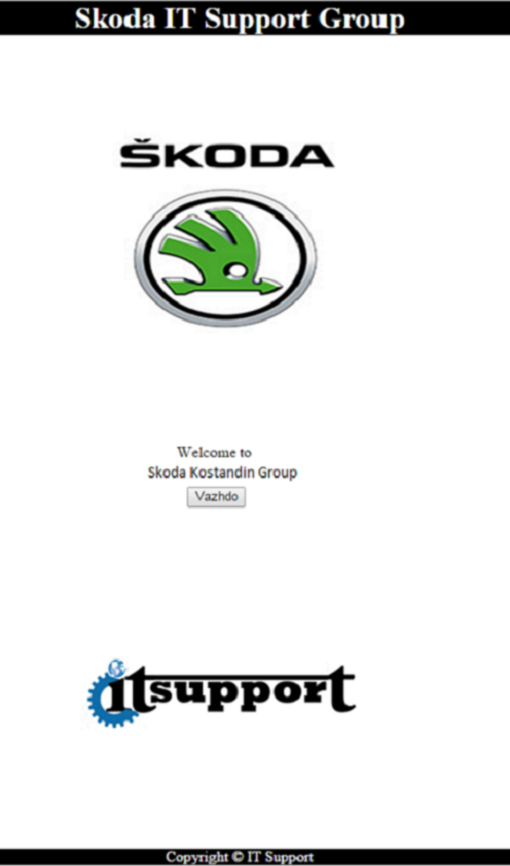
\includegraphics[scale=0.3]{HS2.png}
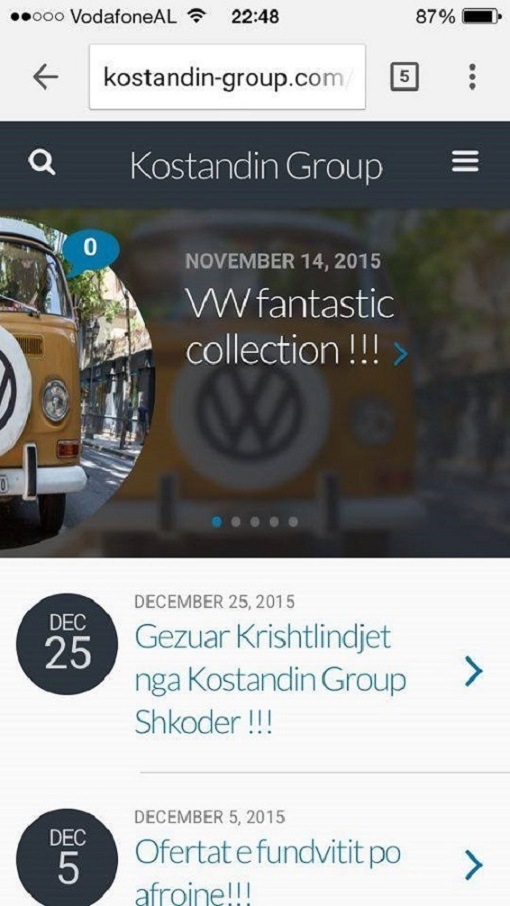
\includegraphics[scale=0.3]{HS3.jpg}

Der Server:
Um die Arbeit der Mitarbeiter der Firma zu erleichtern, haben wir gedacht, ein Server aufzubauen. Die Aufgabe des Server wird die Computers miteinander zu verbinden damit die Mitarbeiter ihre Dateien zentral abspeichern und miteinander teilen. Wir sind noch nicht fertig mit dem Aufbau des Servers aber wir haben den gr\"ossten Teil der Arbeit gemacht und in manche Tagen werden wir fertig sein.

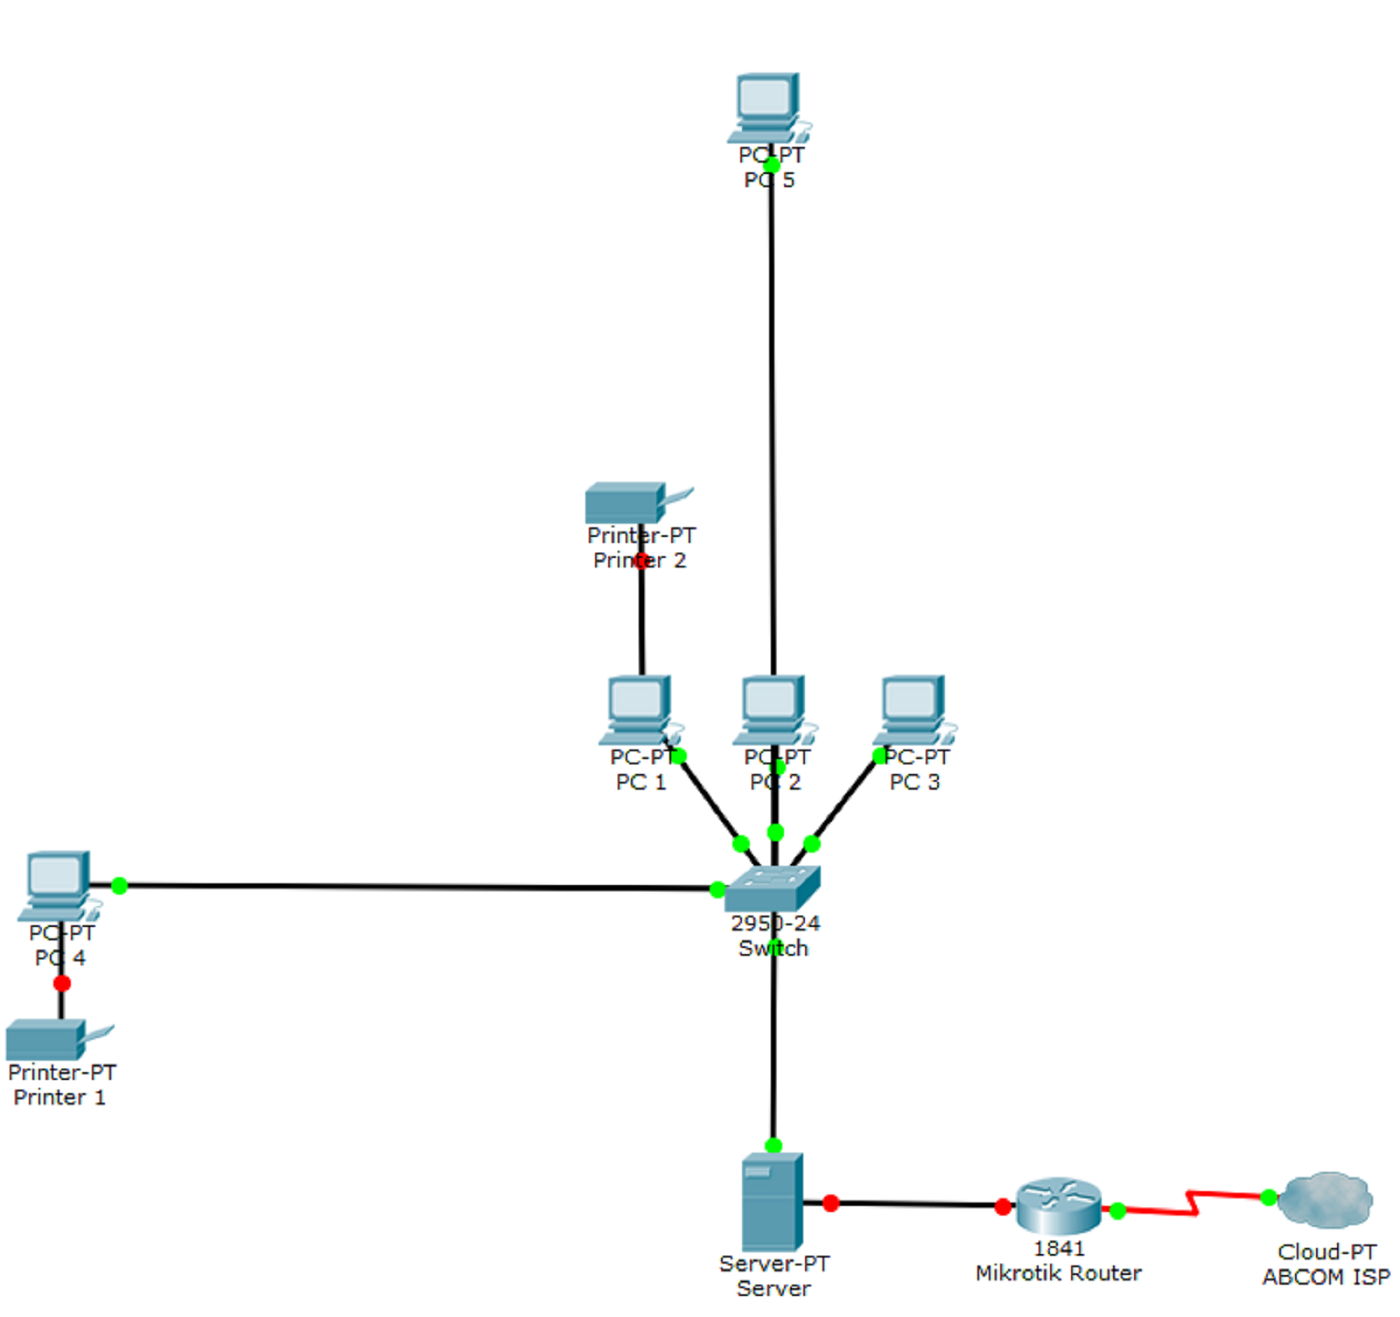
\includegraphics[scale=0.3]{server.png}

Installation und Inbetriebnahme eines Bilanzprogramms, eines Lagerprogramms und eines Rechnungsmanager:
Diese Programme werden die Arbeit der Mitarbeiter viel erleichtern, digitalisieren und schneller Machen. Dort wurden die Kunden gespeichert, die Rechnungen gemacht, alle Teilen gespeicher, der Bilanz jedes Monat gemacht usw. F\"ur die Programme haben wir zwei M\"oglichkeiten: Entweder w\"ahlen wir Open-Sources oder den Programm die von uns erstellt wird. Wir haben unser Programm noch nicht fertig gemacht und nach dem wir es fertig Machen, entscheiden wir, ob wir die Open Sources oder unser Programm verwenden werden

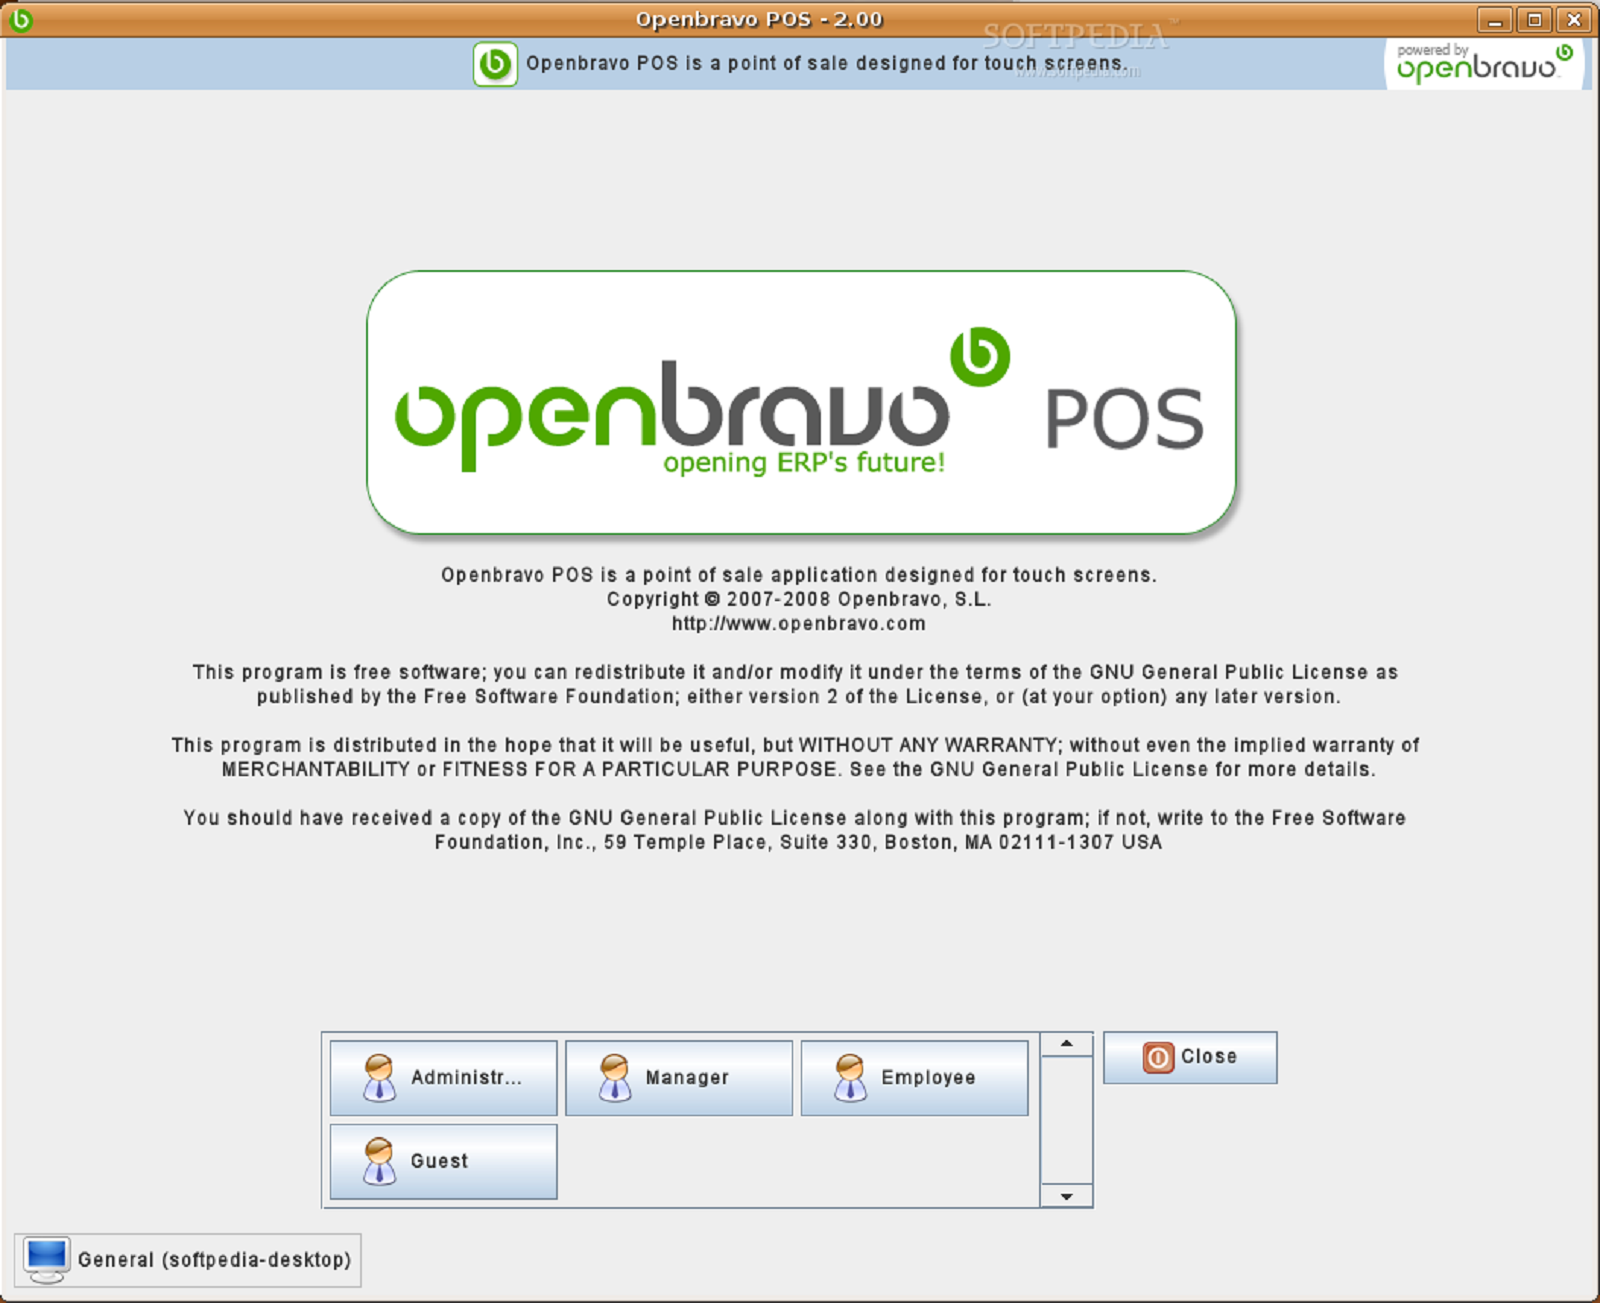
\includegraphics[scale=0.3]{prog1.png} \\
\\
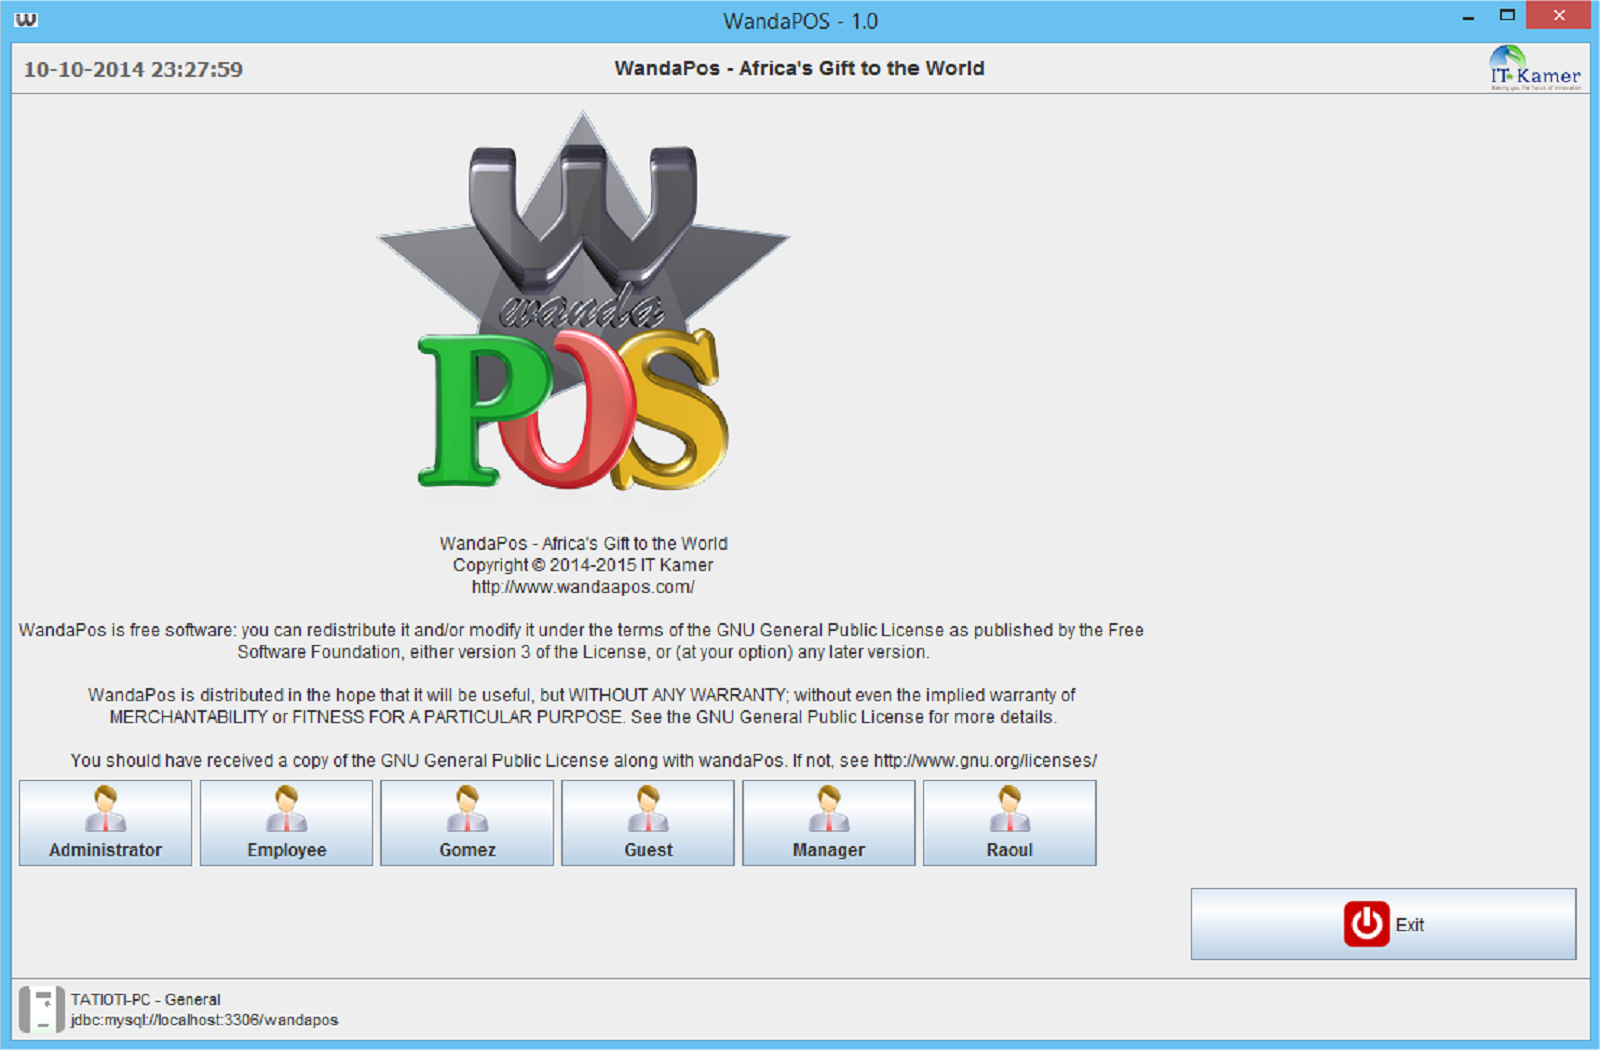
\includegraphics[scale=0.3]{prog2.png} \\
\\
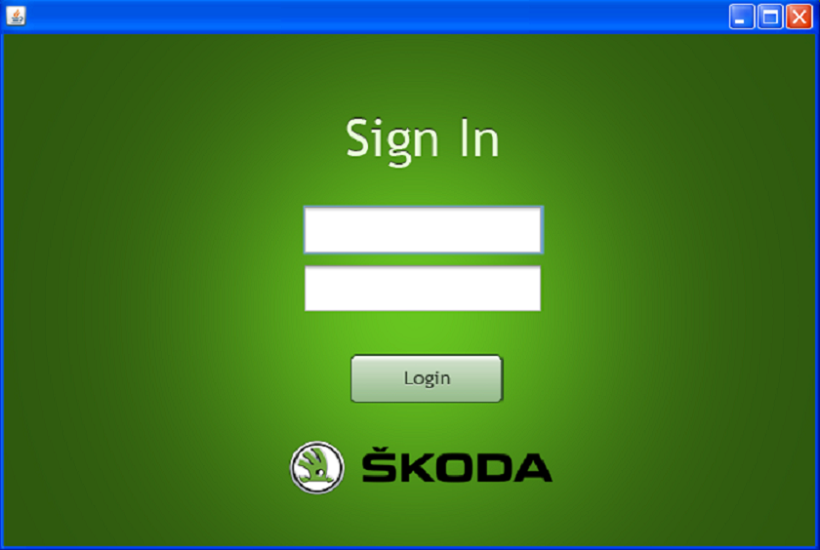
\includegraphics[scale=0.3]{prog5.png}
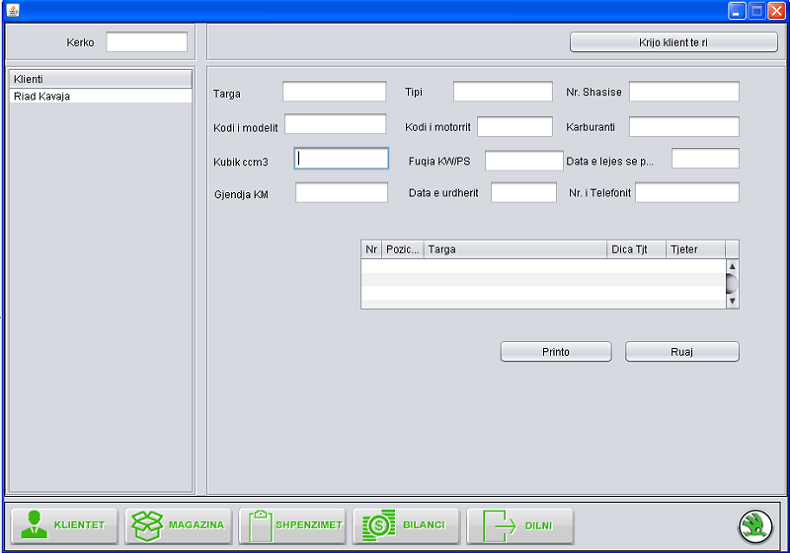
\includegraphics[scale=0.3]{prog6.png} \\
\\
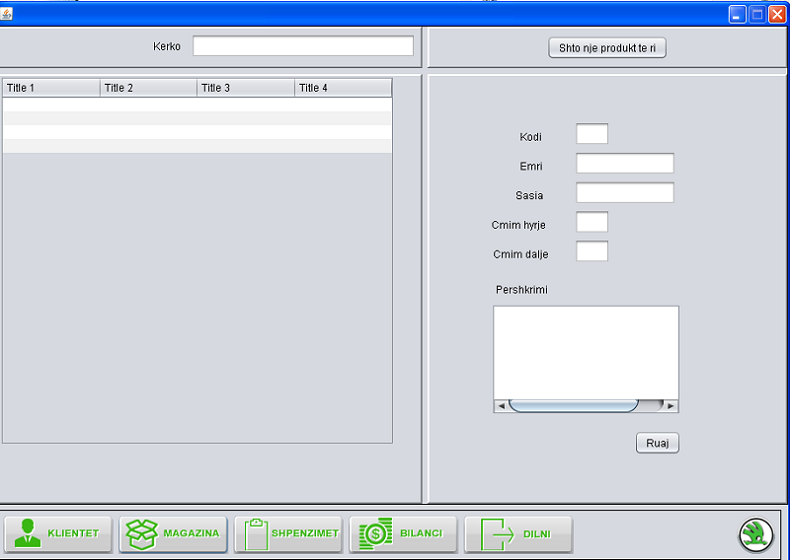
\includegraphics[scale=0.3]{prog7.png} 

Soziale Medien:
Zu Werbezwecken haben wir auch die Soziale Medien gepflegt und verbessert. Wir haben die Facebook-Fanpage verbessert, und Konten in Instagram und Google+ erstellt.

\section{Technische L\"osungen}
\subsection{Webseite}
Um die Website zu erstellen brauchten wir:
\begin{table}[ht]
\caption{Website}
\hspace*{-2cm}
\begin{tabular}{l l}
\hline\hline
Dienste & Preise \\ [0.5ex]
\hline
Domain Namecheap & 10.87 \$ \\
\hline
Host Hostgator & 8.9 \$ pro Monat \\
\hline
Wordpress & Frei \\
\hline
FileZilla & Frei \\
\hline
Themen & Frei \\
\hline
Plugins & Frei \\
\hline
\end{tabular}
\label{table:website} 
\end{table}
\\
Die Webseite haben wir durch diesen Schritte erstellt: \\
Domain wurde von Namecheap gekauft   \\
Host wurde von Hostgator gekauft \\
Wordpress heruntergeladet \\
Mit FTP Verbindung durch Filezilla sind  in Host \\
Database erstellt \\
Wordpress konfiguriert \\
Themes und Plugins installiert \\
CSS verwendet \\
Seite ver\"ofentlicht und Posts hinzugef\"ugt \\

\subsection{Die Hotspot-Zone}
Um die die Hotspot-Zone zu erstellen brauchten wir:

\begin{table}[ht]
\caption{Die Hotspot-Zone}
\hspace*{-2cm}
\begin{tabular}{l l}
\hline\hline
Dienste & Preise \\ [0.5ex]
\hline
Router & 58 euro \\
\hline
USB & 7 euro \\
\hline
DD-WRT & Frei \\
\hline
Notpad++ & Frei \\
\hline
\end{tabular}
\label{table:hotspot} 
\end{table}
Die Hotspot-Zone haben wir durch diesen Schritte erstellt: \\
Den Router gekauft \\
Den geeignetes Version von DDWRT gefunden, heruntergeladen, installiert und konfiguriert. \\
Hotspot erstellt und die Name ge\"andert \\
Die Sicherheits Kode weggenommen. \\
Es wurde so konfiguriert, dass wenn man mit Wireless sich verbindet, wird eine statische Seite ge\"offnet, den wir selbst programmiert haben, und danach automatisch zur Webseite kostandin-group.com springen. \\

\subsection{Netzwerk}
Um die die Netzwerk zu erstellen brauchten wir:

\begin{table}[ht]
\caption{Netzwerk}
\hspace*{-2cm}
\begin{tabular}{l l}
\hline\hline
Dienste & Preise \\ [0.5ex]
\hline
Visio & Frei  \\
\hline
Cisco Packet Tracer & Frei \\
\hline
Visioner 3D & Frei \\
\hline
Server & 100 euro \\
\hline
Windows Server 2008 R2 & Frei \\
\hline
\end{tabular}
\label{table:hotspot} 
\end{table}


\section{Beschreibungen des Arbeitsverlaufs}

Wir haben unser Arbeit gut organisiert, gleich geteilt, und wir haben r\"agelm\"assig gearbeitet, damit wir nicht sp\"at mit die Termine sind. Wir haben jede Mitwoch und Freitag 3 Stunden und nach dem Unterricht manchmal wenn wir etwas schnell machen mochten. Am Wochenenden haben wir auch oft gearbeitet. 
Wir haben Termine mit unserem Projektleiter, Herrn Michel gemacht. Wir haben ihm unseren Arbeit jede Woche pr\"asentiert und er hat uns es zu korrigieren geholfen und neue Ideen und Vorschl\"age gegeben.
Wir haben auch unser Projektauftraggeber getroffen und haben ihm was wir vis jetzt gemacht haben pr\"asentiert, wir haben ihm gefragt ob ihm es gef\"allt und ob er Vorschl\"age hat.
  
\section{Probleme, Herausforderungen und deren L\"osung}

Der Projektauftraggeber hat unsere Plannung ge\"andert, deshalb war es f\"ur uns nicht leicht, den Arbeit noch ein mal zu planen. Der in den ersten Plannung war das Netzwerk, die Programme und dann die Webseite und Pflegen der Sozialen Medien zu absolvieren und die Hotspot- Zone. Danach hat er gesagt dass am Beginn braucht er die Webseite, die Hotspot- Zone und die soziale Medien und danach das Netzwerk und die Programme. Um die Arbeit in der Termin fertig zu machen, haben wir die Arbeit noch einmal geteilt und mehr am begin gearbeitet, damit wir keine Problem mit die Termine am Ende zu haben. 
